\documentclass[aspectratio=169,11pt]{beamer}

\usetheme{Madrid}
\usecolortheme{default}
\usefonttheme{professionalfonts}
\setbeamertemplate{navigation symbols}{}
\setbeamertemplate{footline}[frame number]

\usepackage[T1]{fontenc}
\usepackage[utf8]{inputenc}
\usepackage{lmodern}
\usepackage{microtype}
\usepackage{tikz}
\usetikzlibrary{positioning,arrows.meta}
\usepackage{booktabs}
\usepackage{tabularx}
\usepackage{array}
\usepackage{ragged2e}

\definecolor{Ink}{HTML}{1F2937}
\definecolor{Teal}{HTML}{0F766E}
\definecolor{Mint}{HTML}{CCFBF1}
\definecolor{Gold}{HTML}{F59E0B}
\definecolor{Sky}{HTML}{EFFCFB}
\definecolor{Rose}{HTML}{FFF7ED}
\definecolor{Slate}{HTML}{E5E7EB}

\setbeamercolor{structure}{fg=Teal}
\setbeamercolor{frametitle}{fg=Ink,bg=white}
\setbeamercolor{title}{fg=Ink}
\setbeamercolor{block title}{fg=white,bg=Teal}
\setbeamercolor{block body}{bg=Sky,fg=Ink}
\setbeamercolor{alerted text}{fg=Gold}
\setbeamertemplate{itemize item}{\color{Gold}$\blacktriangleright$}
\setbeamertemplate{itemize subitem}{\color{Teal}$\circ$}
\setbeamerfont{frametitle}{series=\bfseries,size=\Large}

\newcolumntype{Y}{>{\RaggedRight\arraybackslash}X}

\newcommand{\bigidea}[1]{
  \begin{block}{Big idea}
  \Large #1
  \end{block}
}

\title{Teaching AI as a Learning Partner}
\subtitle{A Neurodivergent-Friendly Professional Development Module from My Teaching Placement}
\author{Piter Garcia}
\institute{EDU442 Impacting Practice Roundtable \\ Pine Brook IGNITE Teaching Placement}
\date{Spring 2026}

\begin{document}

\begin{frame}[plain]
\begin{tikzpicture}[remember picture,overlay]
\fill[Sky] (current page.south west) rectangle (current page.north east);
\fill[Teal!12] (0.35,0.45) rectangle (12.95,6.95);
\draw[line width=7pt, color=Gold] (0.65,6.65) -- (12.65,6.65);
\draw[line width=7pt, color=Mint!80!Teal] (0.65,0.75) -- (12.65,0.75);
\end{tikzpicture}
\vspace{0.55cm}
{\huge\bfseries Teaching AI as a Learning Partner\par}
\vspace{0.2cm}
{\Large A neurodivergent-friendly professional development artifact\par}
\vspace{0.15cm}
{\large grounded in my Pine Brook IGNITE teaching placement\par}
\vspace{0.45cm}
\begin{center}
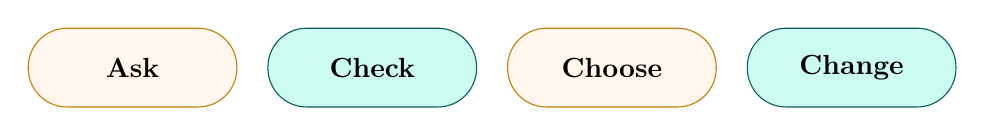
\begin{tikzpicture}[node distance=0.38cm]
\node[rounded corners=14pt, fill=Rose, draw=Gold!80!black, minimum width=2.65cm, minimum height=1cm, align=center] (a) {\bfseries Ask};
\node[rounded corners=14pt, fill=Mint, draw=Teal!80!black, minimum width=2.65cm, minimum height=1cm, align=center, right=of a] (b) {\bfseries Check};
\node[rounded corners=14pt, fill=Rose, draw=Gold!80!black, minimum width=2.65cm, minimum height=1cm, align=center, right=of b] (c) {\bfseries Choose};
\node[rounded corners=14pt, fill=Mint, draw=Teal!80!black, minimum width=2.65cm, minimum height=1cm, align=center, right=of c] (d) {\bfseries Change};
\end{tikzpicture}
\end{center}
\vspace{0.3cm}
\begin{block}{Core claim}
\large Teachers need explicit routines for helping students use AI without losing voice, judgment, or ownership.
\end{block}
\end{frame}

\begin{frame}{What professional problem am I trying to solve?}
\bigidea{Teachers are being asked to use AI in classrooms, but many still need a practical, equity-centered structure for doing it well.}

\vspace{0.2cm}
\begin{columns}[T]
  \column{0.48\textwidth}
  \begin{block}{What I saw in placement}
  \begin{itemize}
    \item strong curiosity about AI
    \item high engagement with digital tools
    \item students moving quickly to whatever the tool produced
  \end{itemize}
  \end{block}

  \column{0.48\textwidth}
  \begin{block}{Why teachers need support}
  \begin{itemize}
    \item tool navigation overshadowing learning
    \item copying without checking
    \item uneven independence
    \item teachers needing a routine they can actually implement
  \end{itemize}
  \end{block}
\end{columns}
\end{frame}

\begin{frame}{Why this matters in EDU442}
\begin{itemize}
  \item EDU442 asks us to turn course ideas about race, class, gender, disability, and equity into a usable practice artifact.
  \item A professional development module is one valid impacting-practice format under the assignment.
  \item In my placement, inclusive teaching often meant balancing \textbf{support} with \textbf{independence}.
  \item That same tension appeared in AI lessons:
  \begin{itemize}
    \item students needed structure to access the tool
    \item but too much teacher rescue reduced agency
  \end{itemize}
  \item This project grew into a PD question: \textbf{How can we help teachers teach AI in ways that support diverse learners without reproducing inequity or replacing student thinking?}
\end{itemize}
\end{frame}

\begin{frame}{Placement evidence that shaped the project}
\small
\begin{tabularx}{\textwidth}{@{}p{3.4cm}YY@{}}
\toprule
\textbf{Source} & \textbf{What it showed} & \textbf{What I learned} \\
\midrule
Responsible AI and Canva Publishing & AI literacy needs chunked routines, visible success criteria, and clear proof of learning. & Students need AI instruction that is structured, not vague. \\
\addlinespace
AI as a Thought Partner & Students benefit when AI is framed as a helper for brainstorming and problem solving. & The language around AI matters. It should support thinking, not replace it. \\
\addlinespace
MagicSchool pilot lesson & Students needed modeling for login, prompts, topic choice, and deciding what to keep from AI output. & Responsible AI use must be explicitly taught. \\
\bottomrule
\end{tabularx}
\end{frame}

\begin{frame}{My impacting practice artifact}
\begin{block}{Artifact}
\Large Professional Development Module: Teaching AI as a Learning Partner
\end{block}

\vspace{0.25cm}
\begin{itemize}
  \item A teacher-facing PD session built from my MagicSchool Student-Choice AI Partner Project
  \item Intended audience: elementary teachers exploring classroom AI use
  \item Main deliverable: a practical framework, model lesson structure, and implementation moves
  \item The PD does not just say ``use AI''
  \item It trains teachers to help students \textbf{plan, check, revise, explain, and stay the author of their own work}
\end{itemize}
\end{frame}

\begin{frame}{What the PD module includes}
\begin{center}
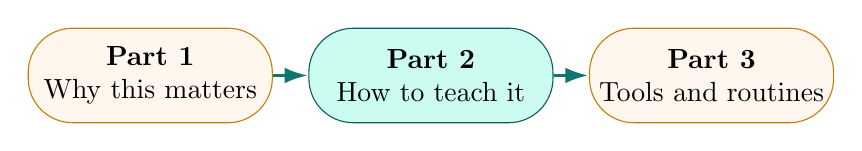
\begin{tikzpicture}[node distance=0.45cm]
\node[rounded corners=16pt, fill=Rose, draw=Gold!80!black, minimum width=3.1cm, minimum height=1.2cm, align=center] (why) {\bfseries Part 1 \\ Why this matters};
\node[rounded corners=16pt, fill=Mint, draw=Teal!80!black, minimum width=3.1cm, minimum height=1.2cm, align=center, right=of why] (how) {\bfseries Part 2 \\ How to teach it};
\node[rounded corners=16pt, fill=Rose, draw=Gold!80!black, minimum width=3.1cm, minimum height=1.2cm, align=center, right=of how] (tools) {\bfseries Part 3 \\ Tools and routines};
\draw[-{Latex[length=3mm,width=2mm]}, line width=1.4pt, color=Teal] (why) -- (how);
\draw[-{Latex[length=3mm,width=2mm]}, line width=1.4pt, color=Teal] (how) -- (tools);
\end{tikzpicture}
\end{center}

\vspace{0.35cm}
\begin{block}{Across all three sessions}
\large Teachers learn a reusable classroom routine: \textbf{Ask, Check, Choose, Change, Explain}
\end{block}
\end{frame}

\begin{frame}{What teachers learn in the PD}
\begin{columns}[T]
  \column{0.48\textwidth}
  \begin{block}{Instructional design moves}
  \begin{itemize}
    \item chunked directions
    \item visible routines
    \item reduced typing load
    \item prompt starters
    \item checkpoints before overload grows
  \end{itemize}
  \end{block}

  \column{0.48\textwidth}
  \begin{block}{Inclusive implementation moves}
  \begin{itemize}
    \item flexible product choices
    \item teacher think-alouds
    \item partner roles
    \item drawing, dictation, or oral rehearsal before typing
    \item support for access without removing ownership
  \end{itemize}
  \end{block}
\end{columns}

\vspace{0.2cm}
\begin{alertblock}{Key principle}
The tool should adapt to the learner. The learner should not have to adapt completely to the tool.
\end{alertblock}
\end{frame}

\begin{frame}{Core message of the PD}
\begin{itemize}
  \item AI can help students brainstorm, narrow a topic, and organize ideas.
  \item It can reduce the blank-page problem for students who struggle to get started.
  \item It can support clearer explanations, simpler language, and step-by-step planning.
  \item For some learners, especially students who need structure or language support, AI can function as a low-stakes thought partner.
\end{itemize}

\vspace{0.25cm}
\begin{block}{But only if...}
\large teachers are prepared to teach questioning, revising, and explaining rather than allowing copy-and-submit use.
\end{block}
\end{frame}

\begin{frame}{What the classroom evidence tells teachers}
\begin{columns}[T]
  \column{0.48\textwidth}
  \begin{block}{What teachers should keep}
  \begin{itemize}
    \item student choice increased buy-in
    \item copyable prompts reduced friction
    \item teacher modeling made safer use possible
    \item partner talk lowered language load
  \end{itemize}
  \end{block}

  \column{0.48\textwidth}
  \begin{block}{What teachers should plan for}
  \begin{itemize}
    \item logging in and tab management took time
    \item some students treated AI output as final
    \item some topics were too broad
    \item success criteria had to remain visible all lesson
  \end{itemize}
  \end{block}
\end{columns}
\end{frame}

\begin{frame}{The deeper instructional shift}
\bigidea{This PD is not about giving teachers one more tool. It is about helping teachers shape how students think with AI while keeping authorship, judgment, and responsibility.}

\vspace{0.2cm}
\begin{itemize}
  \item This is a digital-literacy goal.
  \item This is an inclusion goal.
  \item This is also a future-ready goal for classrooms where AI will increasingly be present.
\end{itemize}
\end{frame}

\begin{frame}{Why this counts as impacting practice}
\begin{itemize}
  \item It is grounded in real teaching-placement experience, not a hypothetical future classroom.
  \item It responds to a recurring instructional need I actually observed.
  \item It produces a reusable PD artifact that another teacher or team could adapt.
  \item It connects educational technology, special education thinking, and responsible instruction.
  \item It moves from reflection to design:
  \begin{itemize}
    \item What did I see?
    \item What problem kept repeating?
    \item What practical teacher support could improve it?
  \end{itemize}
\end{itemize}
\end{frame}

\begin{frame}{What I would add to the PD next}
\begin{itemize}
  \item a facilitator guide with timing and discussion prompts
  \item sample student artifacts from each product type
  \item a teacher-facing checklist for prompt quality, topic fit, and independence
  \item a shorter version for grade-level teams or coaching cycles
  \item a lighter adaptation for younger grades or higher-support settings
\end{itemize}
\end{frame}

\begin{frame}{Closing}
\begin{block}{Final takeaway}
\Large My impacting practice project argues that teachers need PD for AI use that is grounded in visible routines, inclusive scaffolds, and student ownership.
\end{block}

\vspace{0.25cm}
\begin{itemize}
  \item AI should be a learning partner, not a shortcut.
  \item Teacher support should open access, not replace student thinking.
  \item Inclusive structure is what makes responsible AI use possible in real classrooms.
\end{itemize}
\end{frame}

\end{document}
